%\begin{wrapfigure}[0]{r}[-2.5cm]{3cm}
% \vspace{-6cm}
% \includegraphics[scale=0.4]{Schwingkreis/Bilder/schwingkreis.png}
% \vspace{-6cm}
%\end{wrapfigure}

\section*{Theorie- und Prüfungsfragen} 


\mucho{1}{TD203}
{Was ist im Resonanzfall bei der Reihenschaltung einer Induktivität mit einer Kapazität erfüllt?}%Frage
{Der Betrag des induktiven Widerstands ist dann gleich dem Betrag des kapazitiven Widerstands.}%A
{Der Wert des Verlustwiderstands der Spule ist dann gleich dem Wert des Verlustwiderstands des Kondensators.}%B
{Die Größe des elektrischen Feldes in der Spule ist dann gleich der Größe des elektrischen Feldes im Kondensators.}%C
{Die Größe des magnetischen Feldes in der Spule ist dann gleich der Größe des magnetischen Feldes im Kondensator.}%D
{A}%Lösung

\mucho{2}{TD209}
{Welche Resonanzfrequenz hat die Parallelschaltung einer Spule von 2 $\mu H$ mit einem Kondensator von 60 $pF$ und einem Widerstand von 10$k\Omega$?}%Frage
{145,288kHz}%A
{1,45288MHz}%B
{14,5288MHz}%C
{145,288 MHz}%D
{C}%Lösung

\mucho{3}{TD206}
{ Wie ändert sich die Resonanzfrequenz eines Schwingkreises, wenn
1. die Spule mehr Windungen erhält, 2. die Länge der Spule durch Zusammenschieben der Drahtwicklung verringert wird, 3. ein Kupferkern in das Innere der Spule gebracht wird?}%Frage
{Die Resonanzfrequenz wird bei 1. und 2. kleiner und bei 3. größer.}%A
{Die Resonanzfrequenz wird in allen drei Fällen kleiner.}%B
{Die Resonanzfrequenz wird bei 1. kleiner und bei 2. und 3. größer.}%C
{Die Resonanzfrequenz wird bei 1. und 2. größer und bei 3. kleiner.}%D
{A}%Lösung


\mucho{4}{TD201}
{Der Impedanzfrequenzgang in der Abbildung zeigt die Kennlinie\\ 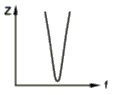
\includegraphics[scale=0.5]{Schwingkreis/Bilder/TD201.png}}%Frage
{eines Serienschwingkreises.}%A
{eines Parallelschwingkreises.}%B
{einer Induktivität.}%C
{einer Kapazität.}%D
{A}%Lösung

\vspace*{0.65cm}

\mucho{5}{TD202}
{Der Impedanzfrequenzgang in der Abbildung zeigt die Kennlinie\\
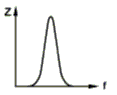
\includegraphics[scale=0.5]{Schwingkreis/Bilder/TD202.png}}%Frage
{eines Serienschwingkreises.}%A
{eines Parallelschwingkreises.}%B
{einer Induktivität.}%C
{einer Kapazität.}
{B}%Lösung

\aufgabentext{
	\begin{enumerate}
	\item[6] Um welche Schaltungen handelt es sich in folgender Abbildung.
	\end{enumerate}
	\loesung{1 Reihenschwingkreis, 2 Parallelschwingkreis, 3 Tiefpass, 4 Hochpass, 5 Bandpass, 6 Saugkreis, 7 Sperrkreis }
	}

\begin{figure}[H]
	\centering
	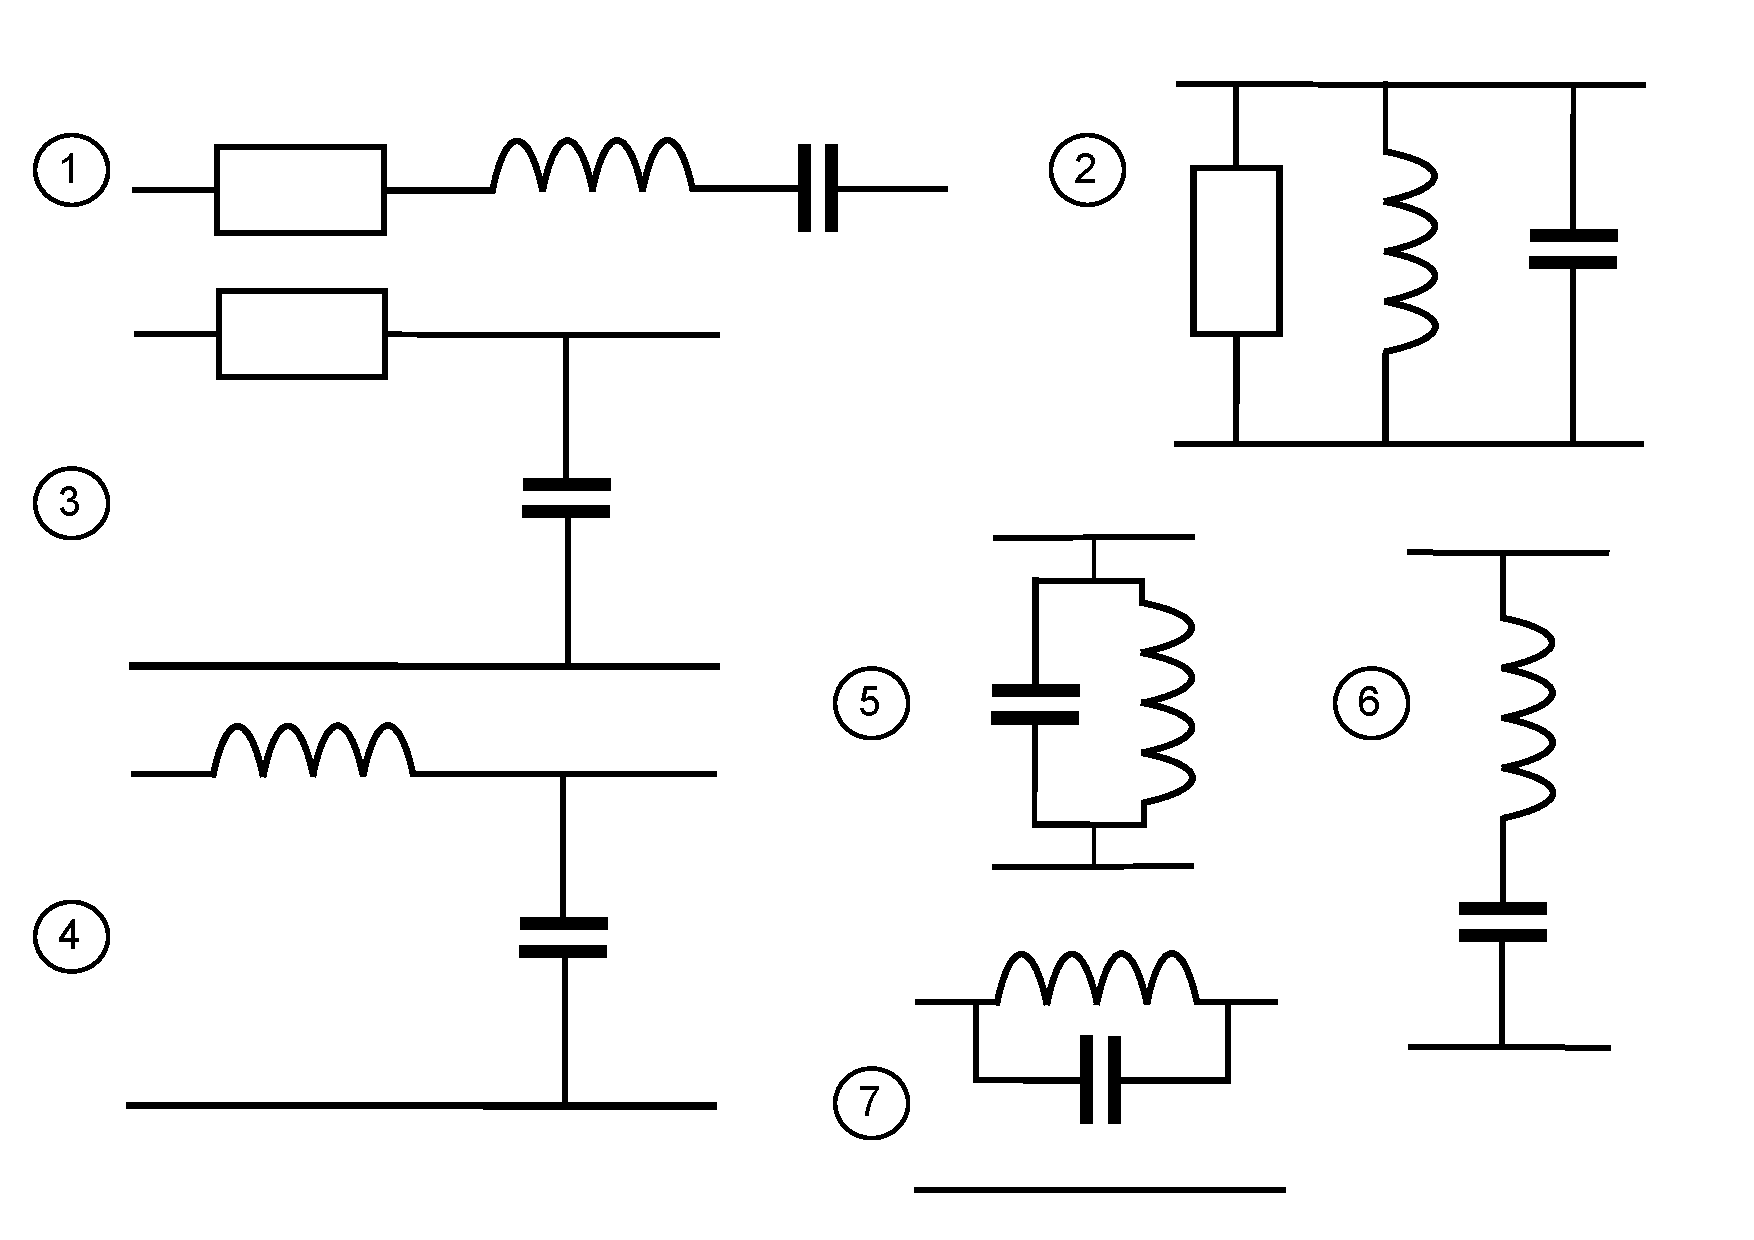
\includegraphics[scale=0.5]{Schwingkreis/Bilder/Filterschaltungen.pdf}
	\end{figure}

\mucho{7}{TD213}
{Welche Grenzfrequenz ergibt sich bei einem RC-Tiefpass mit einem Widerstand von 10$k\Omega$ und einem Kondensator von 50$nF$?}%Frage
{0,32$Hz$}%A
{318$Hz$}%B
{421$Hz$}%C
{318$kHz$}%D
{B}%Lösung
